% exercise sheet with header on every page for math or close subjects
\documentclass[12pt]{article}
\usepackage[utf8]{inputenc} 
\usepackage{latexsym} 
\usepackage{multicol}
\usepackage{fancyhdr}
\usepackage{amsfonts} 
\usepackage{amsmath}
\usepackage{amssymb}
\usepackage{enumerate}
\usepackage{listings}
\usepackage{graphicx}
\usepackage{hyperref}

% Shortcuts for bb, frak and cal letters
\newcommand{\E}{\mathbb{E}}
\newcommand{\V}{\mathbb{V}}
\renewcommand{\P}{\mathbb{P}}
\newcommand{\N}{\mathbb{N}}
\newcommand{\R}{\mathbb{R}}
\newcommand{\C}{\mathbb{C}}
\newcommand{\Z}{\mathbb{Z}}
\newcommand{\Pfrak}{\mathfrak{P}}
\newcommand{\Pfrac}{\mathfrak{P}}
\newcommand{\Bfrac}{\mathfrak{P}}
\newcommand{\Bfrak}{\mathfrak{B}}
\newcommand{\Fcal}{\mathcal{F}}
\newcommand{\Ycal}{\mathcal{Y}}
\newcommand{\Bcal}{\mathcal{B}}
\newcommand{\Acal}{\mathcal{A}}

% formating
\topmargin -1.5cm 
\textheight 24cm
\textwidth 16.0 cm 
\oddsidemargin -0.1cm

% Fancy Header on every Page
\pagestyle{fancy}
\lhead{\textbf{Pattern and Speech Recognition}}
\rhead{Daniel Schäfer (2549458)\\ Christian Bohnenberger (2548364) \\ Dominik Weber (2548553)}
\renewcommand{\headrulewidth}{1.2pt}

\setlength{\headheight}{45pt} 

\begin{document}
\pagenumbering{gobble}

% TODO set the number of the exercise sheet here!
\setcounter{section}{4}

\subsection{k-Means Clustering}
\begin{enumerate}[a)]
    \item 
        Here you can see the provided \verb* data_kmeans.txt  Datapoints
        \begin{center}
            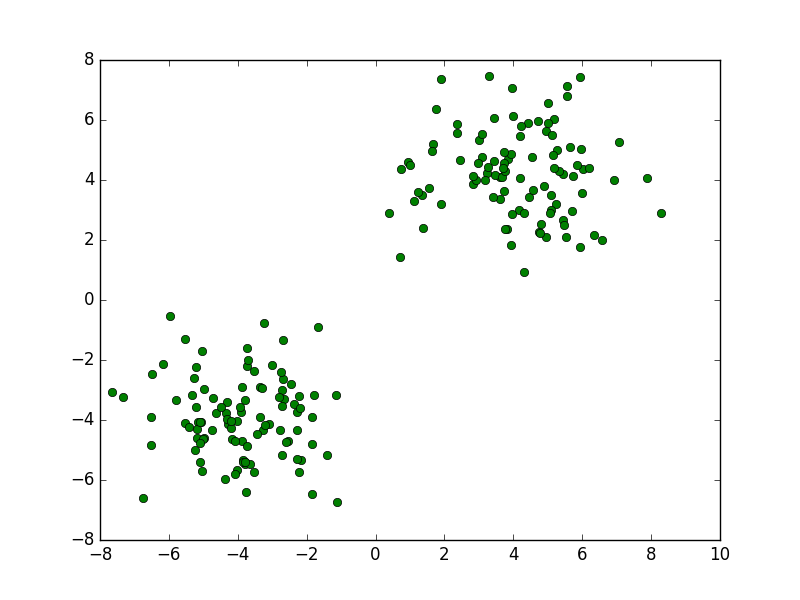
\includegraphics[scale = 0.52]{pictures/datapoints}\\
        \end{center}

    \item 
        see file kmeans.py

    \item 
        Here you can see the clustering steps:
        \begin{center}
            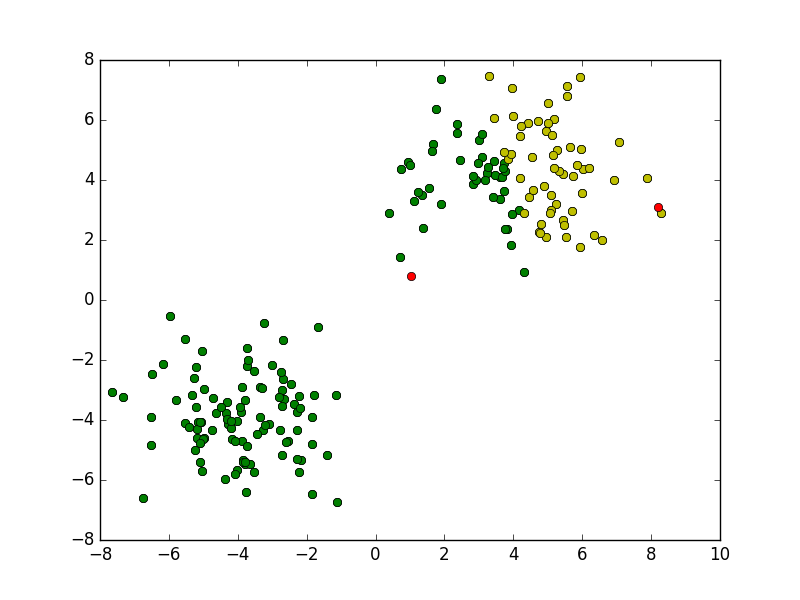
\includegraphics[scale = 0.52]{pictures/plot1}\\
            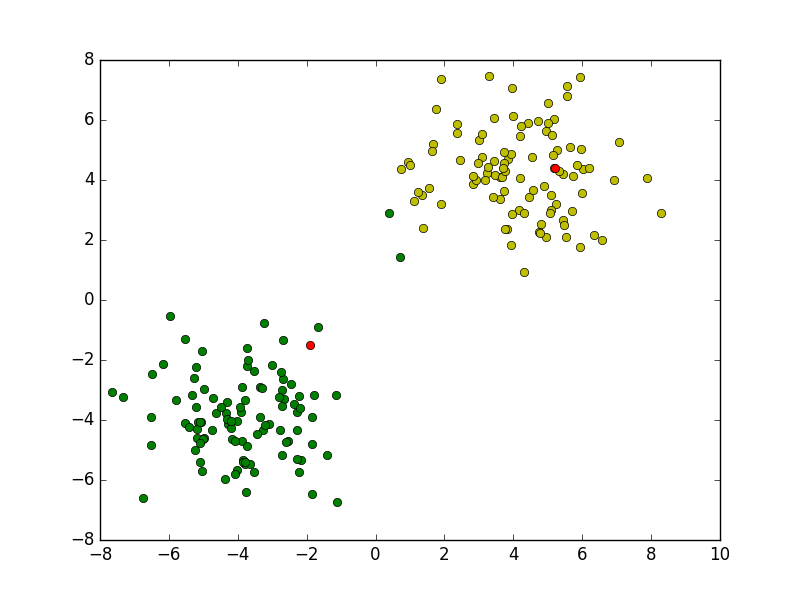
\includegraphics[scale = 0.52]{pictures/plot2}\\
            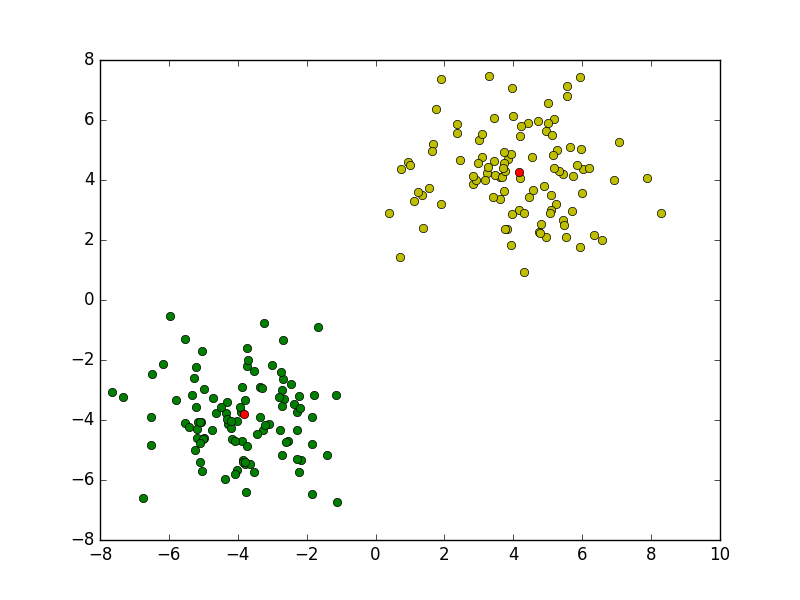
\includegraphics[scale = 0.52]{pictures/plot3}\\
            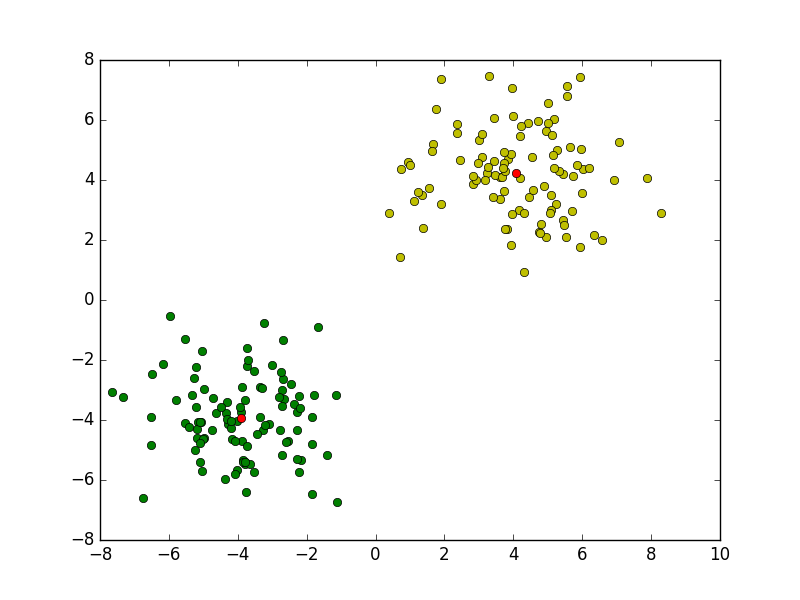
\includegraphics[scale = 0.52]{pictures/plot4}\\
        \end{center}

        the random clusters moved like this:
        \begin{itemize}

            \item 
                \textbf{Picture 1:}\\
                generated random cluster 1 at (1.0221709411131013, 0.7841772734348531)\\
                generated random cluster 2 at (8.213207477643335, 3.0972673201979424)

            \item 
                \textbf{Picture 2:}\\
                Step 1: cluster 1 moved to (-1.908999876156978, -1.4972068985158022)\\
                Step 1: cluster 2 moved to (5.21037564989902, 4.393096131680557)

            \item 
                \textbf{Picture 3:}\\
                Step 2: cluster 1 moved to (-3.8302993963816205, -3.801775709971144)\\
                Step 2: cluster 2 moved to (4.158934618965977, 4.267313391886655)

            \item 
                \textbf{Picture 4:}\\
                Step 3: cluster 1 moved to (-3.917826251367856, -3.921069119340969)\\
                Step 3: cluster 2 moved to (4.0866767936452595, 4.225225019219325)

            \item
                the clusters (and J) didnt change after Step4 and the algorithm terminated

        \end{itemize}

    \item 
        J is essentially the sum of the distances of every single datapoint to the closest cluster of that point. For this distance to become zero you need at least the same number of clusters as datapoints in the set, because every datapoint has to have exactly the same coordinates as a cluster for the distance to the closest cluster to be zero. In the case of \verb* data_kmeans.txt we would need $k \geq 200$ for J to attain the value zero.
        
\end{enumerate}

\subsection{Maximum Likelihood Estimation}

	\begin{enumerate}
	
	\item

	There are 6 independent variables with poisson distribution.
	
	$$L(\lambda)= P(\{X_1=2\} \cap \{X_2=3\} \cap \{X_3=0\} \cap \{X_4=2\} \cap \{X_5=1\} \cap \{X_6=5\})$$
	
	$$\Rightarrow^{independency} L(\lambda)= P(X_1=2) * P(X_2=3) * P(X_3=0) * P(X_4=2) * P(X_5=1) * P(X_6=5)$$
	
	Remember: $P(X=x)= \frac{\lambda^x}{x!}*e^{-\lambda}$
	
	$$L(\lambda)= \frac{\lambda^2}{2!}*e^{-\lambda} * \frac{\lambda^3}{3!}*e^{-\lambda} * \frac{\lambda^0}{0!}*e^{-\lambda} * \frac{\lambda^2}{2!}*e^{-\lambda} * \frac{\lambda^1}{1!}*e^{-\lambda} * \frac{\lambda^5}{5!}*e^{-\lambda} $$
	
	$$ \Leftrightarrow L(\lambda)= \frac{1}{2!*3!*0!*2!*1!*5!} * \lambda^{13} * e^{-\lambda} $$
	
	$$ \frac{\delta L(\lambda)}{\delta \lambda} = \frac{1}{2880}*(13\lambda^{12}*e^{-8\lambda} -8\lambda^{13}*e^{-8\lambda})=0$$
	
	$$ \Leftrightarrow -\frac{e^{-8\lambda}*\lambda^{12}*(8\lambda-13)}{2280} = 0 $$
	
	$$ \Rightarrow \hat{\lambda}=0 \vee \hat{\lambda}=\frac{13}{8} $$
	
	The likelihood function has a max at $\hat{\lambda}=\frac{13}{8}$, therefore the desired $\lambda$ is $\lambda=\hat{\lambda}$.

	\item	
	
	$$ P(X_7=2) = \frac{(\frac{13}{8})^2}{2!} * e^{-\frac{13}{8}} \approx 0.2599985 $$
	
	$ P(X_7=2)$ is at about 26\%.
	
	\end{enumerate}

\subsection{Composite functions}
	$$f(x,y)=log(sin(xy))$$\\
		Idea:\\
		First order derivation:\\
		Use chain rule with $f(x)=log(x)$ and $u=sin(xy)$
	\begin{enumerate}
		\item
		First order derivation:\\
		\begin{enumerate}
		\item
		$$ \frac{\delta}{\delta x} f(x,y)=^{Chain~rule} \frac{\delta}{\delta u}(log(u))* \frac{\delta}{\delta x} sin(xy)
			= \frac{\delta}{\delta u}\frac{ln(u)}{ln(10)} * \frac{\delta}{\delta x} sin(xy) $$ \\
		$$	= \frac{1}{u*ln(10)} * \frac{\delta}{\delta x} sin(xy)) 
			= \frac{1}{u*ln(10)} * y * cos(xy) = \frac{y*cos(xy)}{u*ln(10)} $$
		replace u with $sin(xy)$:
		$$ \frac{\delta}{\delta x} f(x,y) = \frac{y*cos(xy)}{sin(xy)*ln(10)} $$
		
		\item
		$ \frac{\delta}{\delta y} f(x,y)$ analogously \\
		$$ \Rightarrow \frac{\delta}{\delta y} f(x,y) = \frac{x*cos(xy)}{sin(xy)*ln(10)} $$
		
		\end{enumerate}
		
		\item		
		Second order derivation:\\
		\begin{enumerate}
			\item
			$$  \frac{\delta}{\delta xx} f(x,y) =  \frac{\delta}{\delta x} \frac{y*cos(xy)}{sin(xy)*ln(10)}$$\\
			$$ = \frac{(\frac{\delta}{\delta x}y*cos(xy))*sin(xy)*ln(10)-(\frac{\delta}{\delta x} sin(xy)*ln(10))*y*cos(xy)}{sin^2(xy)*ln(10)^2} $$\\
			$$ = \frac{y^2 * (-sin(xy))*sin(xy)*ln(10)-y^2*cos(xy)*ln(10)*cos(xy)}{sin^2(xy)*ln(10)^2}$$
			$$ = \frac{y^2*ln(10)*(-sin^2(xy)-cos^2(xy))}{sin^2(xy)*ln(10)^2} = -\frac{y^2}{sin^2(xy)*ln(10)} $$
		
			\item
			$$  \frac{\delta}{\delta xy} f(x,y) =  \frac{\delta}{\delta y} \frac{y*cos(xy)}{sin(xy)*ln(10)}$$\\
			$$ = \frac{(\frac{\delta}{\delta y}y*cos(xy))*sin(xy)*ln(10)-(\frac{\delta}{\delta y} sin(xy)*ln(10))*y*cos(xy)}{sin^2(xy)*ln(10)^2} $$\\
			$$ = \frac{cos(xy)*sin(xy)*ln(10)+ xy*(-sin(xy))*sin(xy)*ln(10) - xy *ln(10) *cos^2(xy)}{sin^2(xy)*ln(10)^2} $$
			
			$$ = \frac{cos(xy)*sin(xy)- xy*sin^2(xy) - xy *cos^2(xy)}{sin^2(xy)*ln(10)} $$
			\item
			$  \frac{\delta}{\delta yy} f(x,y)$ analogously to $  \frac{\delta}{\delta xy} f(x,y) $ \\
			$$  \frac{\delta}{\delta yy} f(x,y)= \frac{-x^2}{sin^2(xy)*ln(10)}$$
			\item
			$  \frac{\delta}{\delta yx} f(x,y)$ analogously to $ \frac{\delta}{\delta xy} f(x,y) $
			$$  \frac{\delta}{\delta yx} f(x,y) = \frac{cos(xy)*sin(xy)- xy*sin^2(xy) - xy *cos^2(xy)}{sin^2(xy)*ln(10)} $$
		\end{enumerate}
		
	\end{enumerate}

\subsection{Classification}


\end{document}
